\documentclass{cslthse-msc}
\usepackage[utf8]{inputenc}
\usepackage[english]{babel}
\usepackage{amsmath}
\usepackage{amsfonts}
\usepackage{amssymb}
\usepackage{amsthm}
\usepackage{amsmath}
\usepackage{mathtools}
%\usepackage{makeidx}
\usepackage{graphicx}
\usepackage[titletoc, header, page]{appendix}
\usepackage{float}

\usepackage{hyperref}
\usepackage{pdfpages}

\usepackage{diagbox}

\DeclarePairedDelimiter\abs{\lvert}{\rvert}%
\DeclarePairedDelimiter\norm{\lVert}{\rVert}%

%\geometry{showframe}

\author{
	Christian Alexander Oliveros Labrador \\
	{\normalsize \href{mailto:christianol_01@hotmail.com}{\texttt{christianol\_01@hotmail.com}}}
	%\and
	%Camilla Lekebjer \\
	%{\normalsize \href{mailto:Camilla.Lekebjer@cs.lth.se}{\texttt{Camilla.Lekebjer@cs.lth.se}}}
}

\title{Improved Sampling \\for \\Temporal Anti-Aliasing}
\subtitle{A Sobel Improved Temporal Anti-Aliasing}
%\company{The Corporation AB LTD Inc}
\supervisor{Michael Doggett, \href{mailto:michael.doggett@cs.lth.se}{\texttt{michael.doggett@cs.lth.se}}}
%\supervisor{John Deer, \href{mailto:jdeer@company.com}{\texttt{jdeer@company.com}}}
\examiner{Flavius Gruian, \href{mailto:Flavius.Gruian@cs.lth.se}{\texttt{Flavius.Gruian@cs.lth.se}}}

\date{\today}
%\date{January 16, 2015}

\acknowledgements{
If you want to thank people, do it here, on a separate right-hand page. Both the U.S. \textit{acknowledgments} and the British \textit{acknowledgements} spellings are acceptable.

We would like to thank Lennart Andersson for his feedback on this template.

We would also like thank Camilla Lekebjer for her contribution on this template, as well as Magnus Hultin for his popular science summary class and example document.
}

\theabstract{
Anti-aliasing is a key component of modern 3D computer-generated imagery. For Real-Time image generation in applications such as games, it is important to increase the sampling rate per pixel to improve overall image quality. But increasing sampling can be expensive, especially for current Deferred Rendering architectures. An innovative solution to this issue is the Temporal Anti-Aliasing (TAA) technique which combines samples from previous frames with the current frame samples to effectively increase the sampling rate. In this thesis, we will explore methods to improve the quality of TAA by using edge detection, of both color and depth, and triangle indexing to ensure only samples belonging to the current frame pixels are blending together. Our objective is to reduce ghosting and other TAA artifacts created with current implementations. Quality improvement will be evaluated by comparing TAA generated images to ground truth images generated by using much higher sample counts that would not be practical in real-time. The improved TAA was tested using MSE, PSNR, and SSIM against the original implementation and other current Anti-Aliasing techniques. The results obtained showed that the improvements applied to TAA satisfied the expectations, surpassing in quality the other techniques. On average, the PSNR values were around 39 and SSIM values above 0.99.
}

\keywords{TAA, Sobel, Anti-Aliasing, Triangle Indexing, TRAA}

%% Only used to display font sizes
\makeatletter
\newcommand\thefontsize[1]{{#1 \f@size pt\par}}
\makeatother
%%%%%%%%%%


\begin{document}
\makefrontmatter
\chapter[Introduction]{Introduction}
Modern Computer Graphics are based on rendering scenes that are made of objects represented as models composed of primitive polygons, the triangle being the most common one used. This is to take advantage of their simplicity and all their geometric properties to create optimal algorithms to handle their rendering. Triangles are composed of three vertices, each of them which consists of a position and other parameters associated with them, i.e. the color or normals of the triangle, for interpolation. 
 
When we want to render the objects in a scene, we take the vertices and send them to the Rendering Pipeline. There, they are processed and mapped to the pixels of the screen with their respective color.

We have two main uses for this process: Offline Applications, like movies; and Real-time Applications, like video games. Each of them have their requirements and constraints, but for this project, we will only give attention to Real-time Applications.

The focus of this project is to improve Temporal Anti-Aliasing implementation, which is a technique that increases the quality of the images after the process of mapping triangles to pixels by mixing frames previously rendered with current ones.

The main requirement would be to render the highest quality possible representation of the scene, with two main constraints: we must render at least thirty frames per second, with no high frame rate loss; and we must work with a limited amount of memory and bandwidth, because we need to be able to run on an average computer or mobile device.  \cite{Doggett2017EDAN35, Shreiner2011}

\section{Problem Definition}
Temporal Anti-Aliasing (TAA) is a relatively new real-time technique that provides good results without incurring heavy memory or processing power costs of other techniques. Edge detection and triangle indexing techniques appear as good candidates to improve the quality of the technique by reducing the ghosting and blurring unwanted effects created by current implementations of TAA. 

The aim of this thesis is to improve the Temporal Anti-Aliasing technique by using edge detection, of both color and depth, and triangle indexing techniques to reduce blurring and ghosting without decreasing the quality of the rendered image or incurring in heavy memory or processing power costs.  


\section{Related Work}
As the simplest Anti-Aliasing technique, we have Super Sampling Anti-Aliasing (SSAA), it consists on rendering at a higher resolution and then downsampling it to the required resolution. Another technique is the Multi Sample Anti-Aliasing (MSAA), which calculates the color for the final pixel just once \cite{Doggett2017EDAN35}.  We can learn what would become the base of Temporal Reprojection Anti-Aliasing (TAA or TRAA) in the papers Accelerating Real-time Shading with Reverse Reprojection Caching  by Nehab D., Sander P. V., Lawrence J., Tatarchuk N., Isidoro J. R. \cite{Nehab2007}, in which they describe how pixel shaders could use save information and reproject it in the next frame; and Amortized Supersampling by Yang L., Nehab D., Sander P. V., Sitthiamorn P., Lawrence J., Hoppe H. \cite{Yang2009} in which they describe how to use the reprojection of old frames in the current one as a method of real time Anti-Aliasing.

Next, we start to see Post Processing techniques like Fast Approximate Anti-Aliasing (FXAA) by Timothy Lottes \cite{Lottes2009} which uses a form of edge detection to correct aliasing while being compatible with the deferred shading architecture. We also found the Crytek implementation of Temporal Anti-Aliasing (TAA or TXAA) explained by Tiago Sousa on his presentation Anti-Aliasing Methods in CryENGINE 3 \cite{JIMENEZ2011_SIGGRAPH11}.

Enhanced Subpixel Morphological Antialiasing (SMAA) by Jorge Jimenez, Jose I. Echeverria, Tiago Sousa and Diego Gutierrez \cite{Jimenez2012} which uses a more complex edge reconstruction technique while being able to work with SSAA, MSAA and a basic form of TAA.
 
Finally, we have the TRAA implementations of Ke Xu for Uncharted 4 and Lasse Fuglsang for Inside, which implement new advances like the Color Clipping Box and Sharpen Filter. These two last implementations are used as the base of this master thesis.  \cite{Fuglsand2016, XU2016}

\chapter{Technological Background}
In this chapter we will explain which tools were used in this master thesis and why.
\section{C++ and Bonobo Framework}
C++ is a compiled general-purpose programming language with imperative, object-oriented programming and low-level memory management features. It is widely used in Computer Graphics due to its performance, especially on real-time applications, and its wide knowledge base.

The Bonobo Framework is the base of the laboratories of Computer Graphics (EDAF80) and High-Performance Computer Graphics (EDAN35) courses from Lund University. It was developed in C++ and provides a rendering engine that is easy to modify and use.
\section{OpenGL and GLSL}
The Open Graphics Library (OpenGL) is a 2D and 3D computer cross-platform open-source graphics Application Programming Interface (API) that abstracts the programmer from directly interacting with Graphic Processor Units (GPUs) to achieve hardware accelerated rendering. It provides the programmer with a graphics pipeline to use, which is normally implemented through hardware.

OpenGL Shading Language (GLSL) is a high-level shading language that allows programmers greater control of the graphics pipeline without requiring the use of the OpenGL assembly language or hardware-specific languages. 
\section{MATLAB}
MATLAB is a proprietary multi-paradigm numerical computing environment. Commonly used for science, engineering, and economics. It is popular for image processing applications because of its wide library of algorithms for this purpose, including image metrics which are used in this thesis.   

\chapter{Theoretical Background}
In this chapter we will explain all the theoretical information that is the base of this master thesis. From the Computer Graphics Theory to the Image Metrics used.
\section{Rendering Pipeline}
Today’s graphics pipeline can be simplified into three steps: Vertex Shader, which moves the geometry associated with the vertices and prepares them for the next step; Rasterizer, which maps the triangles to pixels in the screen, calculates their visibility and interpolates the parameters of the vertices for each pixel covered by the triangle; and the Pixel (or Fragment) Shader which takes the visual pixels from the Rasterizer and colors them.

\begin{figure}[!hbt]
	\centering
	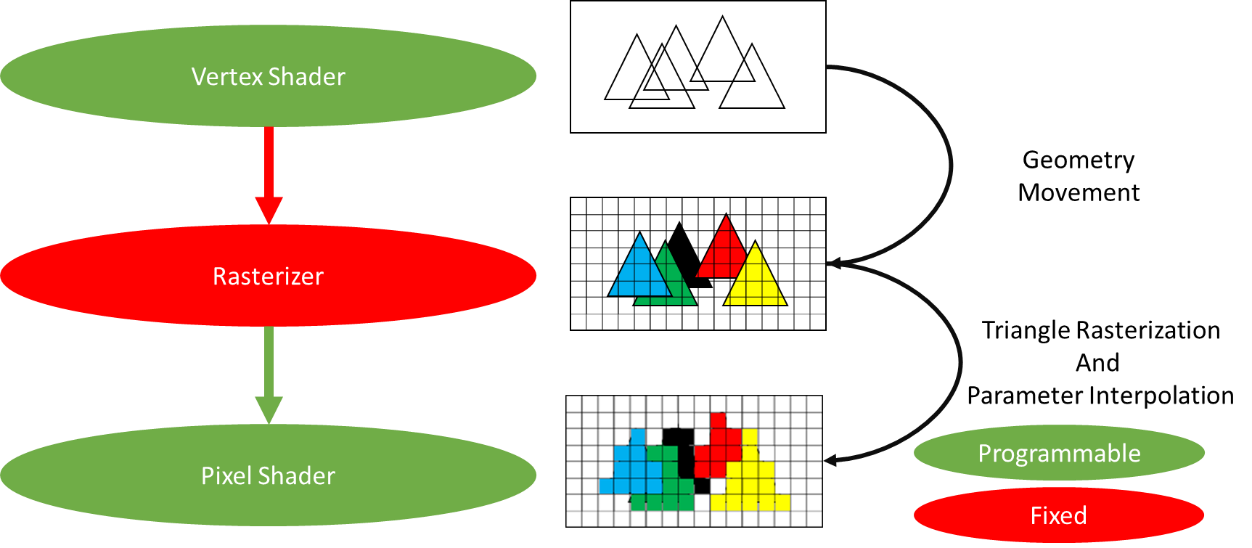
\includegraphics[scale=0.5]{images/graphics_pipeline.png} 
	\caption{Rendering Pipeline, based on EDAF80 5th Lecture.~\cite{Doggett2017EDAF80}}\label{fig:graphpipeline}
\end{figure}

It is important to note that Vertex and Pixel Shaders are controllable by a programmer using special programs called Shaders. They provide a way for the programmer to control the rendering hardware. In contrast, the Rasterizer is not controlled by the programmer and it is handled entirely by a hardware fixed function. \cite{Doggett2017EDAF80}

This Rasterization Process is important for us because it is there where some of the errors corrected by Temporal Anti-Aliasing come from.

\section{Rasterization Process}
During the Rasterization Process, each triangle is tested to establish which pixels are covered by it. While this is being done, each pixel is being tested to find out if another triangle is covering it.

\begin{figure}[!hbt]
	\centering
	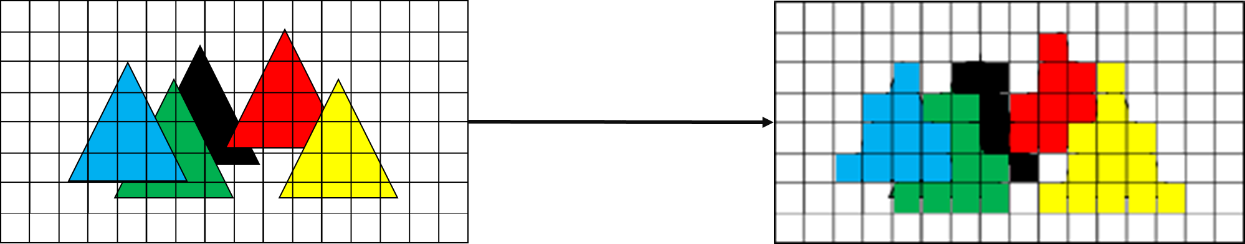
\includegraphics[scale=0.75]{images/rasterization_process.png} 
	\caption{Example of the results of the Rasterization Process.
		\emph{Note}: colors were added to differentiate the triangles, but they would only be added by the Pixel Shader.
	}\label{fig:rasterizationproc}
\end{figure}

Because we are mapping a continuous triangle to a finite number of pixels, we face the problem of pixels partially covered and how to determine whether is enough to qualify it as covered. This is solved by calculating if the center of the pixel is covered by the triangle geometry. This process is susceptible to errors due to the precision of the representation used for the vertices.  

\begin{figure}[!hbt]
	\centering
	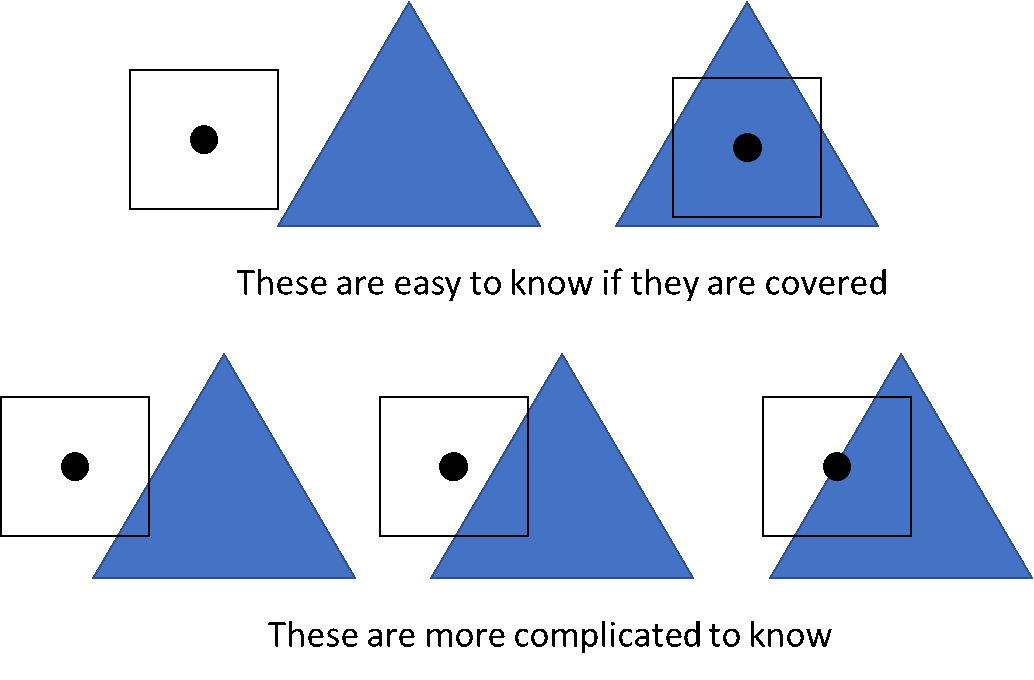
\includegraphics[scale=0.5]{images/edge_testing.png} 
	\caption{Example of the Partial Cover problem, based on EDAN35 second Lecture. ~\cite{Doggett2017EDAN35}}\label{fig:partialcover}
\end{figure}

This process shows us that what is rendered to the screen approximates what is being represented in the scene because pixels can only be covered by one triangle at a time. \cite{Moller2007, Doggett2017EDAN35}

\section{Aliasing Problem}
When we map a continuous representation to a finite one, it is going to generate errors. As explained by Edward Angel and Dave Shreiner in their book (page 413) \cite{Shreiner2011}, we can interpret the rendering process as the sampling of a continuous function $f(x, y)$, which represents the color of the scene at that point, to an $n\times m$  grid of pixels in which we assume that the point $f_{ij}$  is the value of f over a small area; and to reconstruct the $f$ function to display the image to the screen using only what we know from the samples. The mathematical tool used to evaluate the issues of this process is the Fourier Analysis, which states that a function can be decomposed into a set of sinusoids, at possibly an infinite number of frequencies. For two-dimensional image analysis, we can think of the $f$ function as a set of sinusoids at two spatial frequencies.

For this thesis, we will use the First part of the Nyquist sampling theorem as a tool to illustrate why aliasing problems appear and relate to sampling problems. \\

\emph{''Nyquist Sampling Theorem (Part 1): The ideal samples of a continuous function contain all the information in the original function if and only if the continuous function is sampled at a frequency greater than twice the highest frequency in the function.}

\emph{The Nyquist frequency is defined as one half of the sampling frequency, which is the lowest frequency that cannot be in the data to avoid aliasing.''
}

Taken from Edward Angel and Dave Shreiner book page 415. \cite{Shreiner2011} \\

As Edward Angel and Dave Shreiner explain, this idealized sampling assumes that we can take an infinite number of samples per sample frequency which we cannot do in practice. The Aliasing problem that computer graphics experience comes from not being able to sample as required by the Nyquist Sampling Theorem, creating ragged edges that appear in the rasterization process (Spatial Aliasing) and jumps between moving objects (Temporal Aliasing), according to Doggett and Wronski  ~\cite{Doggett2017EDAN35,Wronski2014}. Many solutions have been proposed and used to solve it, e. g. the Super Sampling Anti-Aliasing (SSAA) family of solutions that work on higher frequencies than the required at the cost of more space requirements. 

\begin{figure}[!hbt]
	\centering
	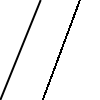
\includegraphics[scale=1.0]{images/aliasing_example.png} 
	\caption{Representation versus Aliased Approximation.}\label{fig:aliasingexample}
\end{figure}

\section[Shadow Mapping and Deferred Shading Architecture]{Shadow Mapping and \\ Deferred Shading Architecture}

As we know, lights and shadows contribute with spatial information to an image. As humans, we have come to expect that objects react to the lights in a scene, considering their geometry; especially because the shadow that it creates gives us a sense of size.

As explained by Michael Doggett \cite{Doggett2017EDAN35}, under the Rendering Pipeline based on the Rasterizer, the process of shadow calculation becomes challenging to do. The Rasterizer does not know if objects are covered or not from a light, so we must figure out a method to calculate if an object is in shadows. 

The shadow calculations are done through a process called Shadow Mapping, it consists of rendering the scene through each light perspective and then test that against the camera perspective to establish if the object is affected by the light or if it is in shadows.

As we might expect, rendering the scene several times is expensive, so we need a way to reduce the cost as much as we can. The Deferred Shading Architecture provides that, it first renders the scene, without light calculations, to a buffer called the Geometry Buffer. There, information regarding colors, normals, depths, specific objects information to interact with lights, etc. is saved so we do not need to recalculate that for each light. After all the information is saved in the Geometry Buffer, we calculate the Shadow Map of every light but only performing depth calculations. Then we calculate the effect of the light using it. In the end, we take all the information of the lights, shadows, and the Geometry Buffer to render the lighted scene.


\section{Anti-Aliasing}
As we have explained, there are two main types of Aliasing, Spatial Aliasing, and Temporal Aliasing; Anti-Aliasing solutions provide improvements against the artifacts created by either of those types at the cost of increased rendering time. For real-time applications this increase of rendering time limits which Anti-Aliasing solutions are feasible to apply.

Another important factor that decides which Anti-Aliasing technique to use is how it behaves with current architectures. For example, old Anti-Aliasing solutions do not work with Deferred Shading.

\subsection{Super Sampling Anti-Aliasing (SSAA)}
As explained by Michael Doggett \cite{Doggett2017EDAN35}, this technique consists in rendering the scene at 4 times the size of the screen and then averaging pixels 4x4 to calculate the result. It provides good results but requires more rendering time and heavy memory usage.

\subsection{Multi Sample Anti-Aliasing (MSAA)}
MSAA consist in taking several samples per pixel; on each sample, the depth values are calculated but only one color is calculated for the rasterized triangle. This solution provides good results at the cost of increased memory usage for depth calculations. 

As explained by Michael Doggett \cite{Doggett2017EDAN35}, the biggest problem this technique has is that it does not work properly with Deferred Shading. This makes it complicated to use with current pipelines, normally requiring other corrections to reduce the artifacts created when applied with Deferred Shading.

\subsection{Fast Approximate Anti-Aliasing (FXAA)}
FXAA is a post-processing anti-aliasing technique that works by detecting edges on the rendered images and then smooth them, as explained by Timothy Lottes. \cite{Lottes2009}

It is relatively cheap compared to MSAA and provides relatively good results, its smoothing capabilities are limited by the amount of information the edge detection can get on a single pass, and it provides relatively good results regarding temporal aliasing.

\subsection{Enhanced Subpixel Morphological Antialiasing (SMAA)}
SMAA is a post-processing technique based on Morphological Anti-Aliasing. It works by reconstructing edges and their surroundings to regenerate the subpixel information lost by aliasing, as explained by Jorge Jimenez, Jose I. Echeverria, Tiago Sousa and Diego Gutierrez. \cite{Jimenez2012}

\section{Temporal Anti-Aliasing}
As explained by Ke Xu and Lasse Fuglsang in their respective presentations ~\cite{Fuglsand2016,XU2016}, the basic principle of Temporal Anti-Aliasing is to mix the current frame being rendered with frames from the past. This is done to increase the number of samples through time rather at the same moment. 

One of such techniques is Temporal Reprojection Anti-Aliasing (TRAA), it works by saving the past frames as a History Buffer which it is then reprojected to the present scene blended to the current frame being rendered.  To do this, we take the current frame and look for the color it should have in the History Buffer, this process is called Reprojection.

To implement TRAA we need: Camera Jitter, Velocity Buffer, Frame History Buffer, Clipping Color Box, Sharpen Filter, and Motion Blur.

\subsection{Camera Jitter}
Camera Jitter is applied every frame to preserve information from local regions of surface fragments. If the current frame is static relative to the past ones then the system is losing information that could be used to refine it. ~\cite{Fuglsand2016,XU2016}

\begin{figure}[!hbt]
	\centering
	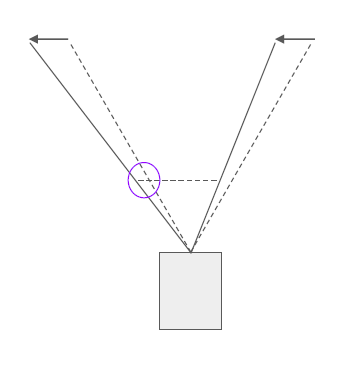
\includegraphics[scale=0.3]{images/camera_jitter.png}
	\caption{Jittering the Projection Process. Image taken from Fuglsand presentation. \protect\cite{Fuglsand2016}}\label{fig:camerajittering}
\end{figure}

The jittering is applied as a translation to the projection matrix using the $Halton Sequence (2,3)$ as the translation deltas. This sequence is used because it generates an irregular pattern for the translations that help preserve more information than a regular pattern and the Halton Sequence provides a cheap pseudorandom pattern generator. ~\cite{Fuglsand2016,XU2016}. 

\begin{figure}[!hbt]
	\centering
	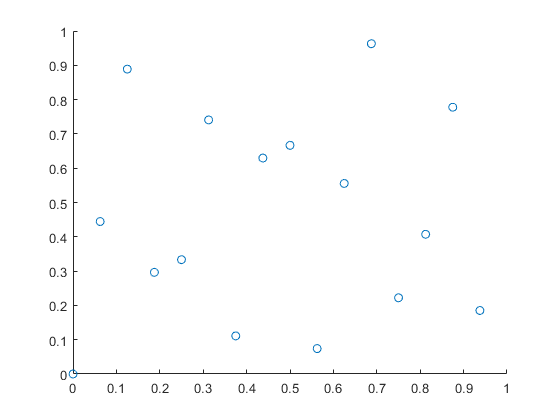
\includegraphics[scale=0.5]{images/halton_16.png}
	\caption{Values from the $Halton Sequence (2,3)$ used.}\label{fig:halton16}
\end{figure}

The Figure~\ref{fig:halton16} shows the representation of the 16 points used to jitter the projection in the current implementation, as proposed by Fuglsand ~\cite{Fuglsand2016}. It was generated using MATLAB with the command \emph{haltonset(2)} then scrambled using reverse-radix scrambling, \emph{scramble(p, 'RR2')} and, finally, generated the 16 points used with \emph{net(p, 16)}.

\subsection{Velocity Buffer}
The Velocity Buffer algorithm used in this implementation is the one proposed by Chapman ~\cite{Chapman2012} which is calculated by subtracting in NDC space the current pixel position by its last frame position. This is possible by saving the MVP matrix of each object in the scene.

Also, as suggested by Xu ~\cite{XU2016}, the jittering is not included as part of the motion.


\subsection{Frame History Buffer}
For each fragment in the current frame, we look for the 3x3 neighborhood and plus $(+)$ pattern neighborhood (See Figure~\ref{fig:samplingpattern}). We look at both patterns for the minimum and maximum of colors of the current frame, next we average them and use it in the Clipping of History ~\cite{Fuglsand2016}.

\begin{figure}[!hbt]
	\centering
	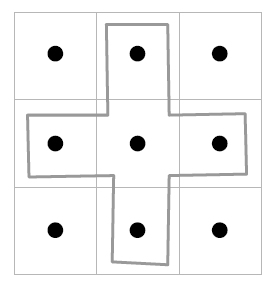
\includegraphics[scale=0.3]{images/sampling_pattern.png}
	\caption{Sampling Pattern used. Image taken from Fuglsand presentation. \protect\cite{Fuglsand2016}}\label{fig:samplingpattern}
\end{figure}

On the $3\times 3$ neighborhood we look for the velocity of the pixel with the closest depth, this is to get better edges in motion for pixels that are occluded ~\cite{Fuglsand2016}. We use this velocity to reproject the position of the current frame in the history. ~\cite{Fuglsand2016,XU2016}

After we have the history, we constrain it (See next subsection) and mix it with the current frame. We linearly mix both using a feedback value that is calculated by the difference of luminance between colors. This feedback is clamped between values closer to one to add some information of the current frame while keeping the history. This mix stabilizes the image, removing the jittering and smoothing the edges ~\cite{Fuglsand2016,XU2016}. Because history is accumulated, we get the effect that each frame weights less the more time the history is not rejected. ~\cite{Fuglsand2016}

\begin{figure}[!hbt]
	\centering
	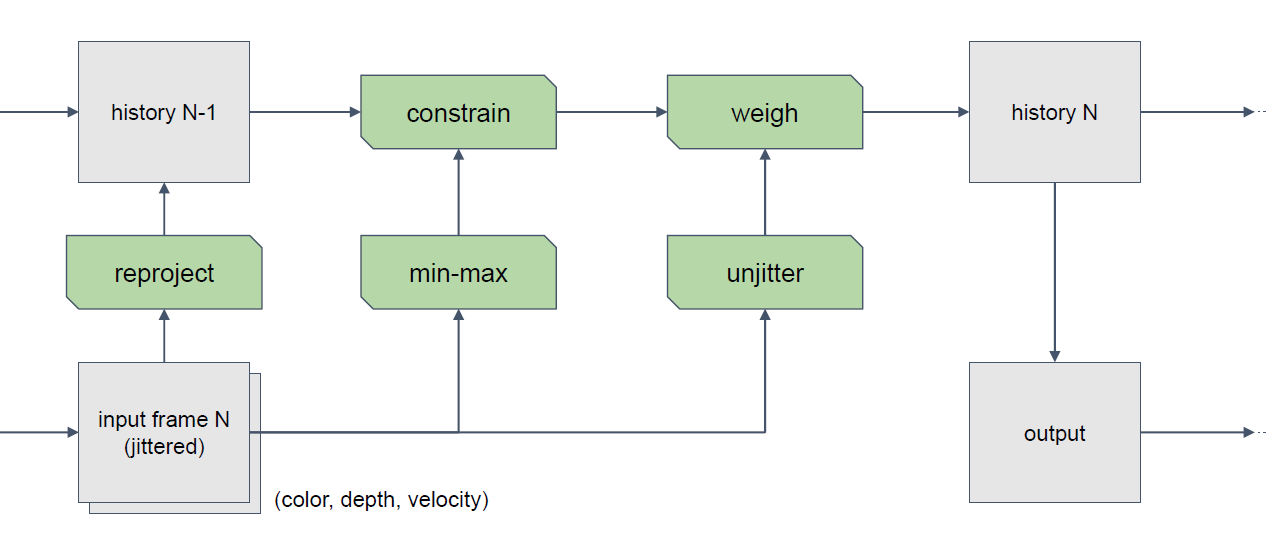
\includegraphics[scale=0.4]{images/sampling_process.png}
	\caption{Temporal Reprojection Anti-Aliasing process. Image taken from Fuglsand presentation \protect\cite{Fuglsand2016}}\label{fig:samplingprocess}
\end{figure}

\subsection{Clipping Color Box} 
A Clipping Color Box is used to handle color rejection when history is too distant from current color. This is a box built using the current pixel color as the center and the minimum and maximum color calculated in the last subsection as limits. The history color is taken as a position and projected against the limits of the box if it lies outside, else, it is left untouched. The usage of the Clipping Color Box prevents the color clustering that would happen if Clamp is applied (See Figure~\ref{fig:clippingbox}). ~\cite{Fuglsand2016}.

\begin{figure}[!hbt]
	\centering
	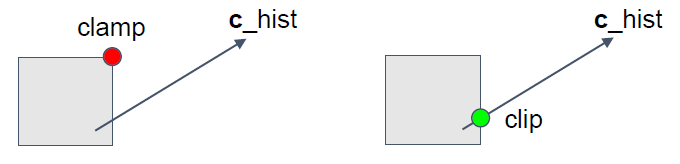
\includegraphics[scale=0.4]{images/clipping_box.png}
	\caption{Color Clamping versus Color Clipping. Image taken from Fuglsand presentation. \protect\cite{Fuglsand2016}}\label{fig:clippingbox}
\end{figure}


\subsection{Sharpen Filter} 
Because the Reprojection process and Color Clipping create blurriness, a Sharpen Filter is required. We used the one proposed by Xu. ~\cite{XU2016}

\begin{equation} \label{eq:sharpen}
\begin{bmatrix*}[r]
0 & -1 &  0 \\
-1 &  5 & -1 \\
0 & -1 &  0
\end{bmatrix*}
\end{equation}

Equation \ref{eq:sharpen} being the Sharpen Filter Convolution Matrix  used in Xu presentation. \protect\cite{XU2016}

\subsection{Motion Blur}
Because the nature of the History Buffer, ghosting is created by fragments from objects that move so fast that they are not rejected as quickly as necessary, under special lighting and background conditions. Fuglsand and Xu ~\cite{Fuglsand2016,XU2016} proposed to use Motion Blur solutions to hide these artifacts.

The Motion Blur used is the one proposed by Chapman ~\cite{Chapman2012}. It tries to behave like a real camera by scaling the velocity of each pixel by the division of the current Frames Per Second (FPS) to the one wanted, thus, simulating the shutter speed. Then it mixes the colors of the pixels that are sampled while following the direction of the velocity buffer vector.

\subsection{Problems}
\subsubsection{Blurriness} 
Current implementations of TAA generate a very aggressive blur because of the way they mix the colors of the current frame and the history; the use of areas larger than the pixel increases the errors generated, therefore a Sharpen Filter is required. The filter applied in the implementation is the one used by Xu ~\cite{XU2016}, it solves blurriness reasonably well but it cannot eliminate some artifacts. 

\subsubsection{Ghosting} 
Some Ghosting is created when objects move, especially under particular lighting and background conditions that make the foreground and background look alike. This is partially corrected with motion blur nevertheless some of it remains near objects that move fast enough to create some Ghosting but slow enough to avoid Motion Blur. Xu proposes the use of Motion Blur and to increase the size of everything using a Stencil technique and manual tagging of objects~\cite{XU2016}. Pederson implementation allows the jitter in the Velocity Buffer calculations to avoid ghosting but it creates some unwanted blurriness ~\cite{Fuglsand2016}. 

\section{Accumulation Buffer}
The Accumulation Buffer is an anti-aliasing technique that consists, according to Paul Haeberli and Kurt Akeley \cite{Haeberli1990}, on rendering the scene several times with camera jittering and then performing a scaled weighted sum of the renderings to generate the current frame.
This is process increases the sampling per pixel and reduces the aliasing effects at the cost of rendering everything several times per frame.

\section{Sobel Operator}
It is an efficiently computable $3\times 3$ isotropic gradient operator, as explained by Irwin Sobel. \cite{Sobel2014}

It works by taking the four-possible simple central gradient estimates in a $3\times 3$ neighborhood and adding them together. The image function is taken as a density/intensity function and the four-possible estimates as orthogonal vectors which are directional derivatives multiplied by a unit vector specifying the derivative’s direction.  The sum of the four-possible simple central gradient estimates is equivalent to the vector sum of the eight directional derivative vectors.

\begin{equation}
\begin{bmatrix*}[r]\label{eq:sobel_neighborhood}
0 & -1 &  0 \\
-1 &  5 & -1 \\
0 & -1 &  0
\end{bmatrix*}
\end{equation}

Let \ref{eq:sobel_neighborhood} be the $3\times 3$ neighborhood and $\abs*{G}$ the magnitude of the directional derivative estimate of the neighborhood.  

The direction of $G$ will be given by the unit vector to the appropriate neighbor. Vector summing causes all the $e$ (center of the $3\times 3$ neighborhood) values to be canceled leaving only the next expression \ref{eq:sobel_simplification}:
\begin{equation}\label{eq:sobel_simplification}
\begin{split}
	G & =\frac{c-g}{4}*\begin{bmatrix*}1 & 1\end{bmatrix*}+\frac{a-i}{4}*\begin{bmatrix*}-1 & 1\end{bmatrix*}+\frac{b-h}{2}*\begin{bmatrix*}0 & 1\end{bmatrix*}+\frac{f-d}{2}*\begin{bmatrix*}1 & 0\end{bmatrix*} \\ & =\begin{bmatrix*}\frac{c-g-a+i}{4}+\frac{f-d}{2} & \frac{c-g+a-i}{4}+\frac{b-h}{2}\end{bmatrix*}
\end{split}
\end{equation}

Then we multiply by $4$, rather divide by $4$, to approximate the value and ensure that we do not lose precision if we perform this with small fixed-point integers. The newly calculated magnitude is sixteen times larger than the original average gradient.

\begin{equation}\label{eq:sobel_approximation}
\begin{split}
G' = 4 * G =\begin{bmatrix*}(c-g-a+i)+(f-d)*2 & (c-g+a-i)*4+(b-h)*2\end{bmatrix*}
\end{split}
\end{equation}

This can be expressed in two weighting matrices. \ref{eq:sobel_x} for the $x$ component and \ref{eq:sobel_y} for the $y$ component.

\begin{equation}
\begin{bmatrix*}[r]\label{eq:sobel_x}
-1 &  0 & +1 \\
-2 &  0 & +2 \\
-1 &  0 & +1
\end{bmatrix*}
\end{equation}

\begin{equation}
\begin{bmatrix*}[r]\label{eq:sobel_y}
+1 & +2 & +1 \\
 0 &  0 &  0 \\
-1 & -2 & -1
\end{bmatrix*}
\end{equation}

For edge-point detection, what is commonly done is compare the magnitude of $G$ against a numeric threshold to mark points as edges. 

\section{Image Metrics}
The process of measuring the quality of an image is a complicated one. As explained by Yusra A. Y. Al-Najjar and Dr. Der Chen Soong \cite{Yusra2012}, we can follow two main methods: subjective or objective. The subjective methods are based on opinions collected from humans and, as one would expect, are considered expensive, difficult to implement and time-consuming to perform. The second kind of methods, the objective ones, are based on mathematical formulas and algorithms to measure the quality of the image without human intervention. For this thesis, we are using objective methods. 

Objectives methods can be categorized into three groups, as described by Yusra A. Y. Al-Najjar and Dr. Der Chen Soong \cite{Yusra2012}:

\begin{itemize}
	\item \textbf{No-Reference:} In which we have no reference image to compare with.
	\item \textbf{Reduced-Reference:} Where we have partially a reference image.
	\item \textbf{Full-Reference:} We have the complete reference image.
\end{itemize}

For computer graphics, the preferred methods are the Full-Reference ones because reference images can be generated using higher quality but bad performing algorithms to render them. The most common metrics used, and the ones used in this thesis, are: Mean Square Error (MSE); Peak Signal-to-Noise Ratio (PSNR); and the Structural Similarity Index (SSIM).

\subsection{Mean Square Error (MSE)}
Based on the average of the squared error between the pixels of the image and the reference.

\begin{equation}\label{eq:mse}
	MSE=\frac{1}{N*M}\sum\limits_{i=0}^{N-1}\sum\limits_{j=0}^{M-1}(Im(i,j)-Ref(i,j))^2
\end{equation}
Where $N,M$ are the width and height of the images and $Im,Ref$ are the pixel of the Image and Reference.

\subsection{Root Mean Square Deviation (RMSD)}
It is the standard deviation of MSE. Also called Root Mean Square Error (RMSE).
\begin{equation}\label{eq:rmse}
RMSE=\sqrt{MSE}
\end{equation}

\subsection{Peak Signal-to-Noise Ratio (PSNR)}
It is based on the mathematical concept of Signal-To-Noise Ratio (SNR) which measures the signal of the image, which is stored as the colors of the pixels for our purposes, against its error compared to the reference. \cite{Yusra2012}

\begin{equation}\label{eq:psnr}
PSNR=10*\log\left(\frac{S^2}{MSE}\right)
\end{equation}

Where $S$ is the maximum value the signal can achieve.In our case it is $255$ because we use 8-bit color channels. 

\subsection{Structural Similarity Index (SSIM)}
SSIM is a widely used image metric that matches human subjectivity and is highly sensitive to degradations in the spatial structure of image luminance, as explained by W.S. Malpica and A.C. Bovik. \cite{Malpica2009}

It requires two images to compare, $X$ and $Y$, and three similarity functions are performed in a sliding $N\times N$ (typically $11\times 11$) gaussian weighted window.

\begin{equation}\label{eq:ssim_components}
\begin{split}
l(x,y) & = \frac{2*\mu_X(x,y)*\mu_Y(x,y)+C_1}{\mu_X^2(x,y)+\mu_Y^2(x,y)+C_1} \\ 
c(x,y) & = \frac{2*\sigma_X(x,y)*\sigma_Y(x,y)+C_2}{\sigma_X^2(x,y)+\sigma_Y^2(x,y)+C_2} \\ 
s(x,y) & = \frac{\sigma_{XY}(x,y)+C_3}{\sigma_X(x,y)+\sigma_Y(x,y)+C_3}
\end{split}
\end{equation}

Where
\begin{equation*}
\begin{split}
\mu_X(x,y) & = \sum\limits_{p=-P}^{P} \sum\limits_{q=-Q}^{Q} w(p,q)*X(x+p,y+q)\\ 
\sigma_X^2(x,y) & = \sum\limits_{p=-P}^{P} \sum\limits_{q=-Q}^{Q} w(p,q)*\lbrack X(x+p,y+q)-\mu_X(x,y) \rbrack^2\\ 
\sigma_{XY}(x,y) & = \begin{split}\sum\limits_{p=-P}^{P} \sum\limits_{q=-Q}^{Q} w(p,q)& *\lbrack X(x+p,y+q)-\mu_X(x,y)\rbrack \\ & *\lbrack Y(x+p,y+q)-\mu_Y(x,y)\rbrack\end{split}
\end{split}
\end{equation*}

Where $w(p,q)$ is a Gaussian weighing function such that $\sum\limits_{p=-P}^{P} \sum\limits_{q=-Q}^{Q} w(p,q)=1$ and $C_1,C_2,C_3$ are small constants that provide stability when the denominator approaches zero. Typically, they are set as follows: 
\begin{equation*}
	C_1=(K_1*L)^2,C_2=(K_1*L)^2,C_3=\frac{C_2}{2}
\end{equation*}

Where L is the dynamic range of the image and $K_1,K_2\ll1$ small constants. At the end, the three similarity functions are combined in the general form: 

\begin{equation}\label{eq:ssim}
SSIM(x,y)=l(x,y)*c(x,y)*s(x,y)
\end{equation}



\chapter{Development}
In this chapter the main work performed in this master thesis.
\section{EDAN35 Project Improvements}
For this master thesis, we decided to use our project from High Performance Computer Graphics (EDAN35) project as the base. During the course, we implemented a Temporal Reprojection Anti-Aliasing technique based on the presentations of Ke Xu and Lasse Fuglsang ~\cite{Fuglsand2016,XU2016}, from the games Inside and Uncharted 4. It proved to be reliable and well documented; and allowed us to put into practice the fundamentals of the technique in an academic environment, providing the base for improvements performed for this master thesis.

The EDAN35 project implementation had errors in the jittering process that were corrected by properly expanding what both implementations meant by camera jittering , see Appendix \ref{appendix:jitter} for a full explanation. The management of the Halton points was redone to accomplish the improved camera jittering with the inclusion of support of up to 128 points to work as the jittering of the Accumulation Buffer (See Figure \ref{fig:halton128}). Note, though, for Temporal Anti-Aliasing only the first 16 points are used as suggested by Ke Xu and Lasse Fuglsang. ~\cite{Fuglsand2016,XU2016}

\begin{figure}[!hbt]
	\centering
	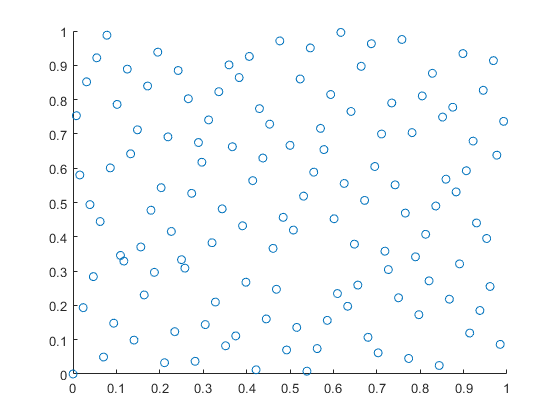
\includegraphics[scale=0.5]{images/halton_128.png}
	\caption{The $128$ $Halton Sequence (2,3)$ Points available to use.}\label{fig:halton128}
\end{figure}

Specular Lighting Anti-Aliasing is a complex problem by itself, which requires specialized solutions that work directly with light reflections. Anti-Aliasing techniques do not correct it by themselves, they usually work with compatible already made solutions. To avoid problems with Specular Lighting, it was decided to be turned off.

Also, there were added models for a sphere, wall, pipe, hairball, a window with blinds and an arched window to test the improvements done to the Temporal Anti-Aliasing. All models, except the wall, were added with one color-solid texture to avoid introducing lighting errors in the calculations of the image metrics for the comparisons between the Uncharted 4 implementation and the one developed in this master thesis. The wall model uses a white texture with black letters on it, this is because letters use hard edges to define their shape and must stay that way after applying any Anti-Aliasing technique.

\subsection{Fast Approximate Anti-Aliasing (FXAA)}
For this master thesis, the white paper version of Fast Approximate Anti-Aliasing (FXAA) by Timothy Lottes \cite{Lottes2009} was used to compare it against Temporal Anti-Aliasing, on the ground that both techniques are Post-Processing Anti-Aliasing and that FXAA is a popular technique used in the industry. It was implemented  under the highest quality preset according to the white paper without taking into consideration the performance impact because we wanted to compare the raw improvement that both techniques can provide.

\subsection{Enhanced Subpixel Morphological Antialiasing (SMAA)}
In order to test a more complex and newer post-processing technique, SMAA was implemented following the instructions provided by Jorge Jimenez, Jose I. Echeverria, Tiago Sousa and Diego \cite{Jimenez2012}. It was implemented using the highest     preset that works with the deferred shading pipeline.

\subsection{Accumulation Buffer}
We use an Accumulation Buffer to provide a reference image of what the scene is. It was implemented following Paul Haeberli and Kurt Akeley \cite{Haeberli1990}. The points used to jitter the camera are Halton Sequence Points as for Temporal Anti-Aliasing, although the Accumulation Buffer can use up to 128. The reasons for using Halton Sequence are that: it fulfils the requirements established by Paul Haeberli and Kurt Akeley; it is easy to extend the current camera system to support more Halton Points; and for Temporal Anti-Aliasing, it provides pseudo-random points that do not follow a pattern to help gather as much information of the scene as possible.

\subsubsection{Sample Number Selection}
The number of samples selected for the Accumulation Buffer is 128. This is because it provides the best representation possible of the scene even though it causes a substantial loss of performance.

In order to show the difference between using 16 and 128 samples, we performed four tests to observe how the metrics behave under different arrangements  of scene objects and lighting. In the next table we see the results of one of such tests:

\begin{table}[!hbt]
	\centering
	\caption{Metrics behavior comparison between using 16 samples versus 128 for Accumulation Buffer.}\label{tab:acctest}
\begin{tabular}{ | l | c | c | c | c | }
	\hline
	\multicolumn{5}{| c |}{Test D} \\
	\hline
	\diagbox{Tests}{Samples}  & \makebox{16} & \makebox{128} & \makebox{Difference} & \makebox{Relative Difference $(\%)$} \\
	\hline
	MSE of Temporal	& $40.647863$ & $38.947297$	& $-1.700566$ & $4.183654132\%$ \\
	RMSD of Temporal & $6.375568$ & $6.240777$ & $-0.134791$ & $2.114180258\%$ \\
	MSE of No AA & $24.872104$ & $24.524992$ & $-0.347112$ & $1.395587603\%$ \\
	RMSD of No AA & $4.987194$ & $4.952271$ & $-0.034923$ & $0.700253489\%$ \\
	Peak-SNR of Temporal & $32.040426$ & $32.22603$ & $0.185604$ & $0.575944353\%$ \\
	SNR of Temporal & $30.30596$ & $30.492374$ & $0.186414$ & $0.611346299\%$ \\
	Peak-SNR of No AA & $34.173678$ & $34.234715$ & $0.061037$ & $0.178289786\%$ \\
	SNR of No AA & $32.439212$ & $32.501058$ & $0.061846$ & $0.190289190\%$ \\
	SSIM of Temporal & $0.993302$ & $0.993451$ & $0.000149$ & $0.014998223\%$ \\
	SSIM of No AA & $0.996826$ & $0.996891$ & $6.5E-05$ & $0.006520272\%$ \\
	\hline		
\end{tabular}
\end{table}

The changes are large enough on some metrics to be noticeable, especially on MSE and SSIM   of Temporal Anti-Aliasing. As for how we are going to notice when we reach the results chapter, these changes are important enough for the comparisons between Anti-Aliasing techniques.

\section{Testing Framework Implementation}
To measure any improvement achieved, we developed a testing framework that allows us to save the important information when the test is performed. The framework allows us to select which technique to use as the main renderer: the master thesis Temporal Anti-Aliasing implementation; Uncharted 4 Temporal Anti-aliasing implementation; Enhanced Subpixel Morphological Antialiasing (SMAA); or Fast Approximate Anti-Aliasing (FXAA). It also allows us to zoom any part of the screen and then perform all the image metrics calculations using MATLAB.
When a test is performed, selected rendered images are saved as PNGs with 4 color channels and no compression. Also, basic information regarding the date when the test was performed; the camera information and data regarding the values used for Temporal Anti-Aliasing are saved in a plain text file.
To quantify if improvements were achieved on the main objectives of this thesis, ghosting, and blurriness, two different types of tests were developed: Static Test and Ghosting Test.

\subsection{Static Test}
This type of test consists of letting the History Buffer fill for 16 frames by rendering them with the Temporal Anti-Aliasing technique selected and then saving the last frame rendered. Immediately rendering the last frame using the Accumulation Buffer, to generate the ground truth image of the scene, and SMAA, FXAA and No Anti-Aliasing (No AA), for comparison purposes. 

\subsection{Ghosting Test}
This type of test is performed only with the sphere and hairball models; the first is moving through the alley of the scene simulating a moving object in an application and the second one is rotating in a static position simulating many edges moving. The test consists of rendering the scene for a selected number of frames, with the Master Thesis Temporal Anti-Aliasing implementation and the Uncharted 4 Temporal Anti-Aliasing implementation at the same time. After each frame is rendered, each image, the position of the sphere and the rotation of the hairball are saved.

Once the selected number of frames has run through, the sphere is returned to its original position and the movement is repeated using the positions saved before; and the hairball is returned to its original rotation and the movement is also repeated. The difference this time is that every frame is rendered using the Accumulation Buffer and then saved, it is done to avoid the heavy performance loss caused by the Accumulation Buffer impacting the Temporal Anti-Aliasing techniques.

\subsection{MATLAB Image Metrics}
Once all the test results are saved, one script takes all the images and organizes them into folders by name and type of test. Afterward, all the test results are processed using MATLAB.

For Static Tests, we perform MSE, RMSD, PSNR, SNR and SSIM measurements to the TAA, FXAA, SMAA and No AA rendered images, using the Accumulation Buffer rendered images as the reference to compare with. Also, we generate a local SSIM map for each rendered image, apart from the one rendered with the Accumulation Buffer, which are saved as PNGs and MATLAB FIGs. All the measurements results are stored in the folder with the test results as a plain text. 

For Ghosting Tests, we perform MSE, RMSD, PSNR, SNR and SSIM measurements to each frame rendered with the Temporal Anti-Aliasing of Uncharted 4 technique and the Temporal Anti-Aliasing of the master thesis using the corresponding Accumulation Buffer rendered frame. A local SSIM map is generated for each rendered image, except the Accumulation Buffer ones, and saved as PNGs and MATLAB FIGs. All the results of all images are stored in a plain text file. In this SSIM maps, dissimilarity is represented as colors and white as similarity.


\section[Temporal Reprojection Anti-Aliasing Modifications]{Temporal Reprojection \\ Anti-Aliasing Modifications}
For this thesis, the Color Clipping Box technique was modified to be affected by the values calculated from the new techniques applied in this thesis. These changes follow the rationale that we want to apply the full force of the Temporal Anti-Aliasing technique when needed, and not elsewhere, to minimize the effects of ghosting and blurring.

The first change consists in that the Colors that were calculated from the average between the $3\times 3$ and Cross neighborhoods by the sampling patterns are now mixed in a variable amount. This follows the idea that we prefer the Cross neighborhood over the $3\times 3$ neighborhood if the pixel we are currently calculating is not considered to be aliased, this is because the Cross neighborhood is less likely to introduce unwanted information in the minimum, maximum and average calculations. But, if the pixel is considered to be aliased, we prefer the $3\times 3$ neighborhood because it provides more information about the surroundings of the pixel to create the unaliased image. 

\begin{figure}[!hbt]
	\centering
	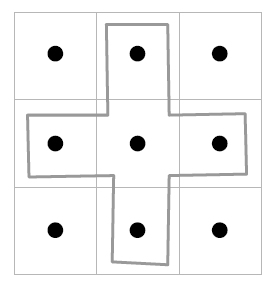
\includegraphics[scale=0.3]{images/sampling_pattern.png}
	\caption{Sampling Pattern used. Image taken from Fuglsand presentation. \protect\cite{Fuglsand2016}}\label{fig:samplingpattern_2}
\end{figure}

The second change consists in that the size of the Color Clipping Box depends on how much the pixel is considered to be aliased. By using small Color Clipping boxes on unaliased pixels, we increase the elimination of unwanted colors from the history, reducing the effects of ghosting since we are rejecting colors faster on pixels that we know are not considered be aliased. This is implemented by linearly interpolating the current pixel color and the minimum and maximum colors calculated for the Color Clipping Box.

\begin{figure}[!hbt]
	\centering
	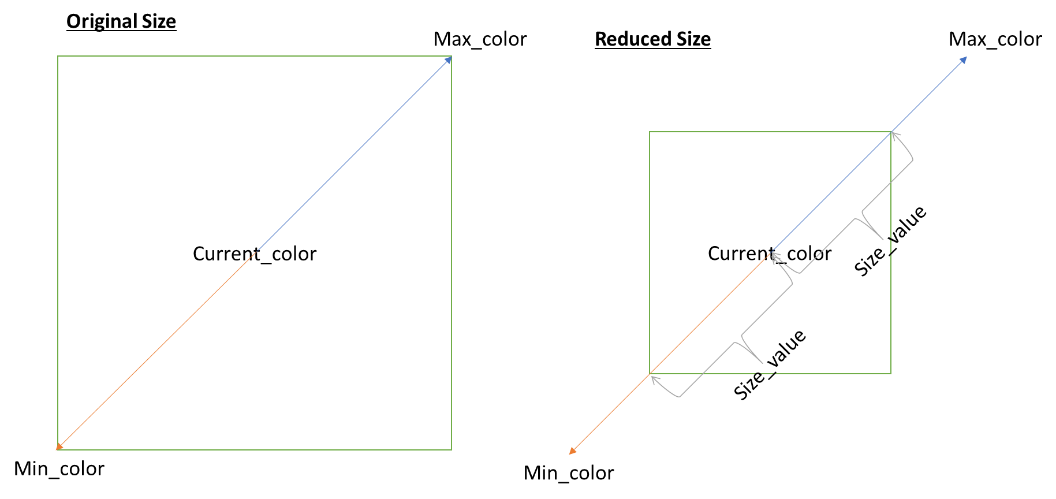
\includegraphics[scale=0.7]{images/clipping_box_reduction.png}
	\caption{Color Clipping Box size reduction}\label{fig:colorclippingboxredux}
\end{figure}

\subsection{Triangle Indexing Improvements Implementation}
The main idea behind the application of this technique is to detect pixels that we considered aliasing by using how many different models one pixel is surrounded with to edges between models. Once we have this information, we proceed to alter the Color Clipping Box that controls the application of TAA.

To implement this technique, all models in the scene receive a unique integer index. Then, in the renderization geometry pass, all triangles belonging to the same model receive the model index as its ID. Subsequently, it is used in the pixel shader to generate a texture in which every pixel contains the ID of the model it belongs to.

On the Temporal Reprojection pass, the average on the number of pixels belonging to different models in the $3\times 3$ neighborhood of the current pixel is calculated. With this average, we proceed to skew the color linear interpolation between the minimum, maximum and average between the Cross and $3\times 3$ neighborhoods of the pixel and we proceed to change the size of the Color Clipping Box. 

If the average is close to zero, meaning that the pixel is surrounded by pixels of its same model, we interpolate towards colors from the Cross neighborhood and reduce the size of the Color Clipping Box. But, if the average is close to one, meaning that the pixel is surrounded by many pixels of other models, we interpolate towards colors from the $3\times 3$ neighborhood and let the Color Clipping Box stay on its original size.

\begin{equation}\label{eq:model_index_acc}
modelAverage_i = \frac{\sum\limits_{j=1}^{9} ModelDiff(i,j)}{9} 
\end{equation}

Where
\begin{equation*}
ModelDiff(i,j) = \left\lbrace \begin{split}1\quad & if\quad ModelID_i \neq ModelID_j \\ 0\quad & else\end{split} \right.
\end{equation*}

\subsection{Depth Pseudo-Variance and Depth Temporal Pseudo-Variance}
The key point behind this technique is that we want to detect pixels that we consider aliased because they are in a neighborhood of pixels separated by relatively long depth distances or that they change their depth relatively a long distance through frames. 

First, we calculate the minimum, maximum and average linear depth from the $3\times 3$ neighborhood. Then we proceed to use the next formula to calculate the value we are going to use to normalize results:
\begin{equation} \label{eq:maxdepthdistance}
\begin{split} 
	maxDepthDistance = min \left( \right. & \left| depthMin-depthAvg \right|  ,   \\ 
	 &  \left.\left| depthMax-depthAvg\right| \right) 
\end{split} 
\end{equation}

We calculate the normalizing value using the minimum to avoid the interference of outliers. If $maxDepthDistance$  is below $0.002$ everything that follows is set to zero because pixels are so close that it’s probably not aliased. This threshold was defined by experimenting which values would not get noise inside the calculations but would let the interesting pixels in. 

Then we calculate the depth pseudo variance as:

\begin{equation} \label{eq:depthpseudovariance}
	depthPseudoVariance = \left( \frac{\left|currentDepth-depthAvg\right|}{maxDepthDistance}\right)^2
\end{equation}

This provides us with a pseudo-variance that measures the distance between the average depth and the current pixel depth. Note that normally the value is going to be between $0$ and $1$ and but, if the pixel depth is an outlier, this value is going to be over $1$.

Finally, we calculate how relates the depth of the pixel in the last frame to the current neighborhood, using the depth temporal pseudo variance. Note that we use the fourth power to reduce the noise in the calculations.

\begin{equation} \label{eq:depthtemporalpseudovariance}
depthTemporalPseudoVariance = \left( \frac{\left|pastDepth-depthAvg\right|}{maxDepthDistance}\right)^4
\end{equation}

\subsection{Sobel Improvements Implementation}
The main idea behind applying Sobel edge detection technique is to concentrate the TAA effects on pixels on edges to correct aliasing, if necessary.  

We apply the Sobel Operator to the luminance of the lighted scene produced by the Deferred Shading Pipeline, the luminance of the unlighted scene from the Geometric Buffer and the current linear depth. We use luminance because the human eye is better at recognizing sudden changes on it and we use the lighted and unlighted scene to avoid problems detecting edges because of lights or shadows.

Each Sobel Operator is performed separately, and their magnitudes mixed at the end as follows:
\begin{equation} \label{eq:sobel_g}
	g=(u*0.3 +l*0.7)+d 
\end{equation}

Where $u$ is the magnitud of the sobel operator of the luminance of the unlighted scene, $l$ is the magnitud of the sobel operator of the luminance of the lighted scene and $d$ is the magnitud of the sobel operator of the current linear depth. \\

Then, we clamp $g$ between $0.0$ and $1.0$ to finally apply the smoothstep polynomial as follow:
\begin{equation} \label{eq:sobel_sqrt}
sobel=\sqrt{g^2*(3.0-2.0*g)} 
\end{equation}

After all the Sobel Operators are applied, we save the results to a texture and perform a simplified version of TRAA to keep the results stable through time. This simplified version is almost the same as the one we use as a base of this master thesis, the differences come from the use Clamping rather than a Clipping Box because the texture values are one dimensional; and we do not apply a sharpen filter.

The output of this TRAA is used to calculate the Sobel value of the current pixel, the average Sobel value in the Cross Neighborhood and the average Sobel value in the $3\times 3$ Neighborhood.

\subsection{Final Mixing}
Finally, we use the values previously calculated to modify how the Clipping Box is calculated.

First , we define the mix function as follows:
\begin{equation} \label{eq:mixfunction}
Mix(x,y,t)=x*(1-t)+y*t\quad with\; 0\leq t\leq 1
\end{equation} 

Then, the final mixing is applied as follows:
\begin{equation}\label{eq:sobelavgmixval}
sobelAvgMixVal=Clamp01(modelAverage_i+sobel) 
\end{equation}
 
Where $sobel$ is the Sobel value of the current pixel, Equation \ref{eq:sobel_sqrt}, $modelAverage_i$ comes from the Equation \ref{eq:model_index_acc} and $Clamp01$ is the clamping function between $0$ and $1$. \\

\begin{equation}\label{eq:sobelavg}
sobelAvg=Mix(sobelAvgCross, sobelAvg3x3, sobelAvgMixVal)
\end{equation}

Where $sobelAvgCross$ is the average Sobel value of the Cross Neighborhood and $sobelAvg3x3$ is the average Sobel value of the $3\times 3$ Neighborhood around the current pixel. \\ 

And, we use Equations \ref{eq:sobelavg}, \ref{eq:depthpseudovariance}, \ref{eq:depthtemporalpseudovariance} and \ref{eq:model_index_acc} to calculate how much this pixel is considered to be aliased:
\begin{equation}\label{eq:aliasedvalue}
\begin{split}
aliasedValue=Clamp01 (& sobelAvg + depthPseudoVariance \\
 & + depthTemporalPseudoVariance \\
 & + modelAverage_i)
\end{split}
\end{equation}

With this $aliasedValue$ we proceed to modify the Color Clipping Box. First, we change how the colors are calculated:
\begin{equation}\label{eq:newcolors}
\begin{split}
colorMin= & Mix(colorMinCross,colorMin3x3,aliasedValue) \\
colorMax= & Mix(colorMaxCross,colorMax3x3,aliasedValue) \\
colorAvg= & Mix(colorAvgCross,colorAvg3x3,aliasedValue) \\
\end{split}
\end{equation}

Then we modify the size of the box:
\begin{equation}\label{eq:clipredux}
\begin{split}
	clipColoorMin= & Mix(colorCurrent,colorMin,aliasedValue) \\
	clipColorMax= & Mix(colorCurrent,colorMax,aliasedValue)
\end{split}
\end{equation}



The Figures \ref{fig:aliasedval1}, \ref{fig:aliasedval2} and \ref{fig:aliasedval3} are examples of the aliased values calculated. The white color represents a value of $1$ and the black color of $0$.

\begin{figure}[H]
	\centering
	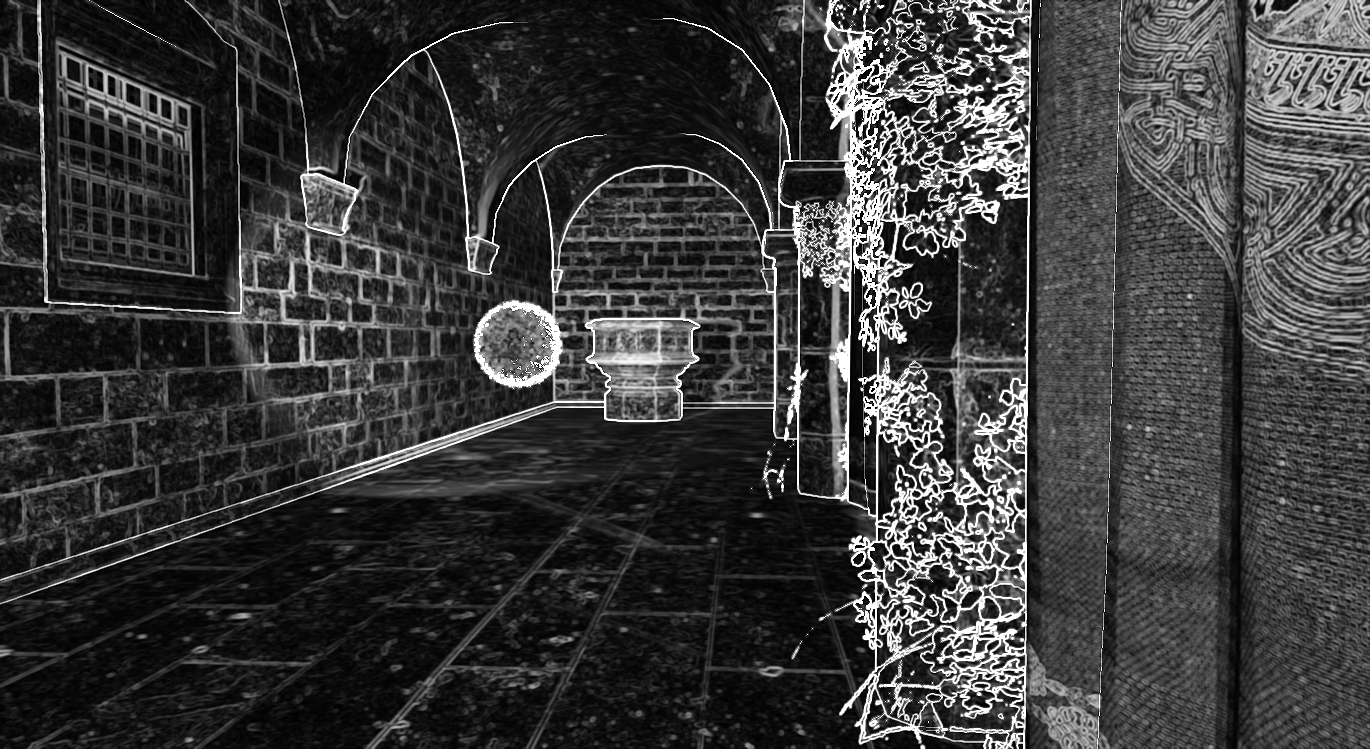
\includegraphics[scale=0.2]{images/aliased_value_example_1_temporal.png}
	\caption{Image made of the Aliased Values of each pixel.}\label{fig:aliasedval1}
\end{figure}

\begin{figure}[H]
	\centering
	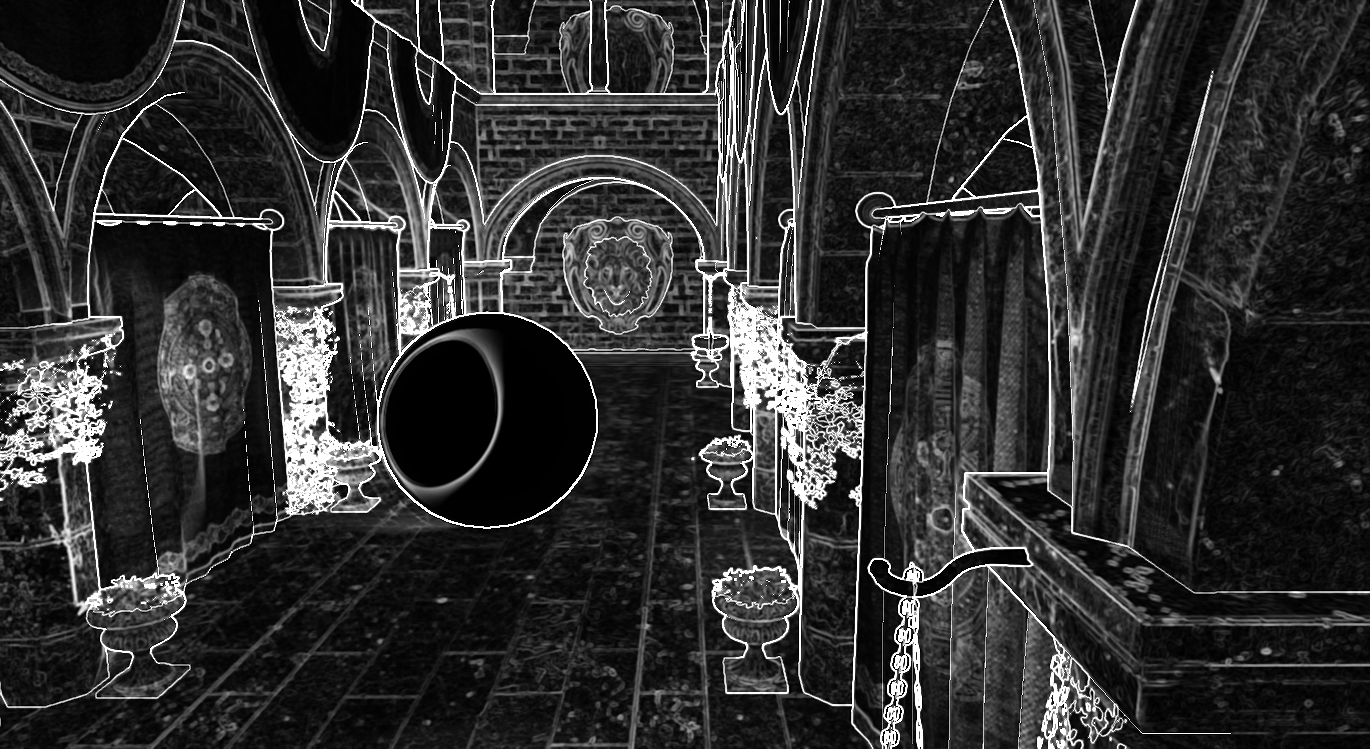
\includegraphics[scale=0.2]{images/aliased_value_example_2_temporal.png}
	\caption{Image made of the Aliased Values of each pixel.}\label{fig:aliasedval2}
\end{figure}

\begin{figure}[H]
	\centering
	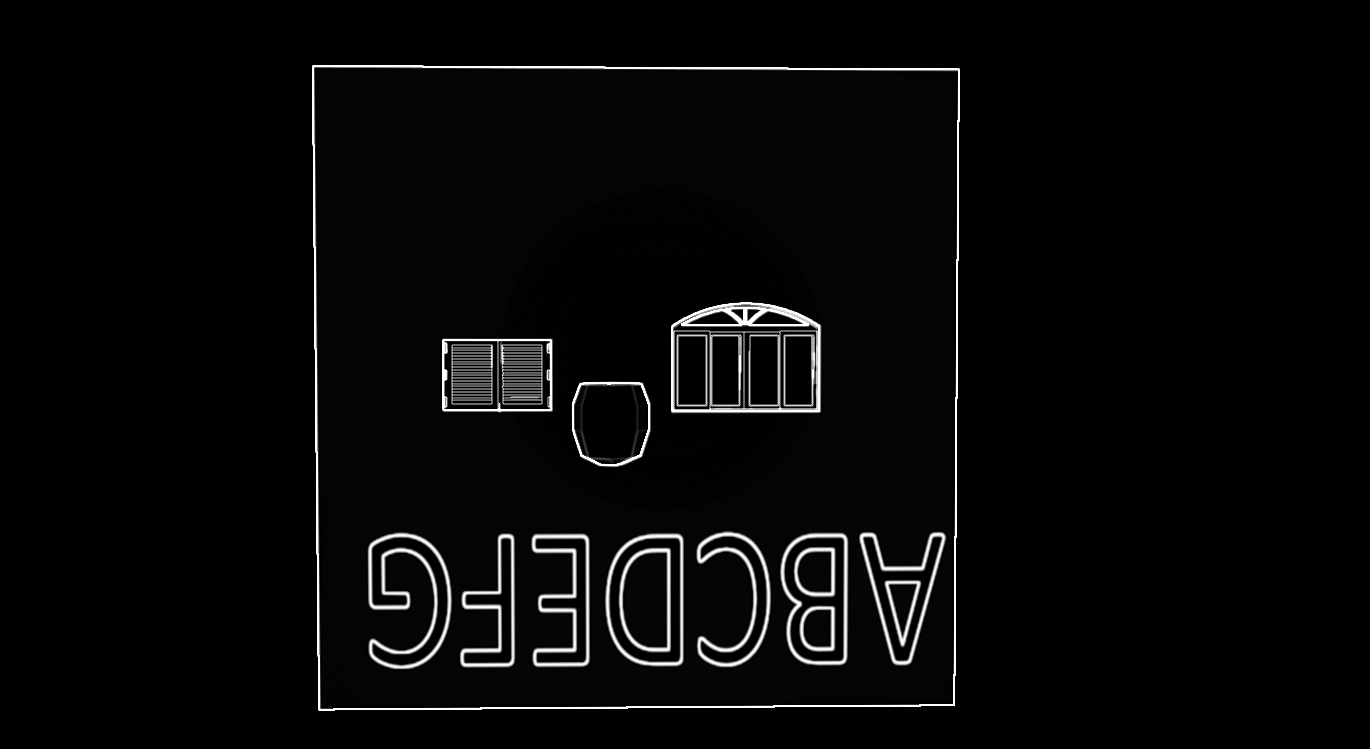
\includegraphics[scale=0.2]{images/aliased_value_example_3_temporal.png}
	\caption{Image made of the Aliased Values of each pixel.}\label{fig:aliasedval3}
\end{figure}

\subsection{Sharpen Filter Modifications}
The Sharpen Filter was normalized to avoid creating a color peak. It was changed from \ref{eq:sharpen} to:
\begin{equation} \label{eq:new_sharpen}
\centering
\begin{bmatrix*}[c]
0 & -0.25 &  0 \\
-0.25  &  2 & -0.25  \\
0 & -0.25  &  0
\end{bmatrix*}
\end{equation}

Equation \ref{eq:new_sharpen} shows the new Sharpen Filter Convolution Matrix used.


\chapter{Results}
In this chapter we explain how we evaluated the improvements done to the Temporal Anti-Aliasing. We show the numerical and visual results obtained. Finally, we explain said results and their meaning compared to the previous implementation of TAA and other Anti-Aliasing solutions.
\section{Evaluation Methodology}
To evaluate the improvements done to the Temporal Anti-Aliasing technique we selected models and camera angles that put the technique under stress. Then, using the Testing Framework we developed, we proceed to render and save images of each of those models to compare how the technique behaves in comparison to the original TAA implementation and other Anti-Aliasing techniques to see if the changes we proposed provided images with better quality without incurring in heavy memory usage or time consumption. Also, an especial test was taken to measure if changing the Sharpen Filter was the only thing providing an improvement.

The tests were performed on the computer provided by Lund University which has the next specification:

\begin{itemize}
\item CPU: Intel(R) Core(TM) i7-3820 CPU @ 3.60GHz, 3601 Mhz, 4 Cores, 8 Logical Processors
\item RAM: 64,0 GB	
\item GPU: NVIDIA GeForce GTX 1080 with 8 GB of VRAM
\item Rendering Resolution when not zooming: 1600 x 900
\end{itemize}



\chapter[Short on Formatting]{Formatting}
Avoid empty spaces between \textit{chapter}-\textit{section}, \textit{section}-\textit{sub-section}. For instance, a very brief summary of the chapter would be one way of bridging the chapter heading and the first section of that chapter.
\section{Page Size and Margins}
Use A4 paper, with the text margins given in Table \ref{tab:margins}.
\begin{table}[!hbt]
\centering
\caption{Text margins for A4.}\label{tab:margins}
\begin{tabular}{cc}
\hline
\textbf{margin} & \textbf{space} \\
\hline 
top &  3.0cm\\ 

bottom & 3.0cm \\ 
 
left (inside) & 2.5cm \\ 

right (outside) & 2.5cm \\ 

binding offset & 1.0cm \\ 
\hline 
\end{tabular} 
\end{table}

\section{Typeface and Font Sizes}
The fonts to use for the reports are \textbf{TeX Gyre Termes} (a \textbf{Times New Roman} clone) for serif fonts, \textsf{\textbf{TeX Gyre Heros}} (a \textsf{\textbf{Helvetica}} clone) for sans-serif fonts, and finally \texttt{\textbf{TeX Gyre Cursor}} (a \texttt{\textbf{Courier}} clone) as mono-space font. All these fonts are included with the TeXLive 2013 installation. Table \ref{tab:fonts} lists the most important text elements and the associated fonts.
\begin{table}[!hbt]
\caption{Font types, faces and sizes to be used.}\label{tab:fonts}

 \begin{tabular}{ l c c c}
\hline 
\textbf{Element} & \textbf{Face} & \textbf{Size}  & \textbf{\LaTeX size}  \\ 
\hline 
{\huge \textbf{Ch. label}} & {\huge \textbf{serif, bold}} & \thefontsize\huge & \verb+\huge+ \\ 
{\Huge \textbf{Chapter}} & {\Huge \textbf{serif, bold}} & \thefontsize\Huge & \verb+\Huge+ \\ 
{\LARGE \textsf{\textbf{Section}}} & {\Large \textsf{\textbf{sans-serif, bold}}} & \thefontsize\LARGE &  \verb+\LARGE+  \\ 
{\Large \textsf{\textbf{Subsection}}} & {\Large \textsf{\textbf{sans-serif, bold}}} & \thefontsize\Large & \verb+\Large+ \\ 
{\large \textsf{\textbf{Subsubsection}}} & {\Large \textsf{\textbf{sans-serif, bold}}} & \thefontsize\large &  \verb+\large+ \\ 
Body & serif & \thefontsize\normalsize & {\footnotesize \verb+\normalsize+} \\
%{\footnotesize Footnote} & serif  & \thefontsize\footnotesize & {\footnotesize \verb+\footnotesize+} \\
{\footnotesize \textsc{Header}} & {\footnotesize \textsc{serif, SmallCaps}} & \thefontsize\footnotesize &  \\
Footer (page numbers) & serif, regular & \thefontsize\normalsize &  \\
\hline
\textbf{Figure label} & \textbf{serif, bold} & \thefontsize\normalsize & \\
Figure caption & serif, regular & \thefontsize\normalsize & \\
\textsf{In figure} & \textsf{sans-serif} & \textit{any} & \\
\textbf{Table label} & \textbf{serif, bold} & \thefontsize\normalsize & \\
Table caption and text & serif, regular & \thefontsize\normalsize & \\
\texttt{Listings} & \texttt{mono-space} & $\le$ \thefontsize\normalsize & \\
\hline 
\end{tabular} 
\end{table}

\subsection{Headers and Footers}
Note that the page headers are aligned towards the outside of the page (right on the right-hand page, left on the left-hand page) and they contain the section title on the right and the chapter title on the left respectively, in \textsc{SmallCaps}. The footers contain only page numbers on the exterior of the page, aligned right or left depending on the page. The lines used to delimit the headers and footers from the rest of the page are $0.4 pt$ thick, and are as long as the text.

\subsection{Chapters, Sections, Paragraphs}
Chapter, section, subsection, etc. names are all left aligned, and numbered as in this document. 

Chapters always start on the right-hand page, with the label and title separated from the rest of the text by a $0.4 pt$ thick line.

Paragraphs are justified (left and right), using single line spacing. Note that the first paragraph of a chapter, section, etc. is not indented, while the following are indented.

\subsection{Tables}
Table captions should be located above the table, justified, and spaced 2.0cm from left and right (important for very long captions). Tables should be numbered, but the numbering is up to you, and could be, for instance:
\begin{itemize}
\item \textbf{Table X.Y} where X is the chapter number and Y is the table number within that chapter. (This is the default in \LaTeX. More on {\LaTeX} can be found on-line, including whole books, such as \cite{goossens93}.) or
\item \textbf{Table Y} where Y is the table number within the whole report
\end{itemize}
As a recommendation, use regular paragraph text in the tables, bold headings and avoid vertical lines (see Table \ref{tab:fonts}). 

\subsection{Figures}
Figure labels, numbering, and captions should be formed similarly to tables. As a recommendation, use vector graphics in figures (Figure \ref{fig:vectorg}), rather than bitmaps (Figure \ref{fig:rasterg}). Text within figures usually looks better with sans-serif fonts.
\begin{figure}[!hbt]
\centering

\includegraphics[scale=2.5]{examplepic1.pdf} 
\caption{A PDF vector graphics figure. Notice the numbering and placement of the caption. The caption text is indented 2.0cm from both left and right text margin.}\label{fig:vectorg}
\end{figure}

\begin{figure}[!hbt]
\centering

\includegraphics[scale=2.5]{examplepic3.jpg} 
\caption{A JPEG bitmap figure. Notice the bad quality of such an image when scaling it. Sometimes bitmap images are unavoidable, such as for screen dumps.}\label{fig:rasterg}
\end{figure}
For those interested in delving deeper into the design of graphical information display, please refer to books such as \cite{Tufte:1986, few2012show}.

\section{Mathematical Formulae and Equations}
You are free to use in-text equations and formulae, usually in \textit{italic serif} font. For instance: $S = \sum_i a_i$. We recommend using numbered equations when you do need to refer to the specific equations:
\begin{equation}
E = \int_0^{\delta} P(t) dt \quad \longleftrightarrow \quad E = m c^2
\end{equation}
The numbering system for equations should be similar to that used for tables and figures.

\section{References}
Your references should be gathered in a \textbf{References} section, located at the end of the document (before \textbf{Appendices}). We recommend using number style references, ordered as appearing in the document or alphabetically. Have a look at the references in this template in order to figure out the style, fonts and fields. Web references are acceptable (with restraint) as long as you specify the date you accessed the given link \cite{fontspec, CTAN}. You may of course use URLs directly in the document, using mono-space font, i.e. \url{http://cs.lth.se/}.

\section{Colours}
As a general rule, all theses are printed in black-and-white, with the exception of selected parts in selected theses that need to display colour images essential to describing the thesis outcome (\textit{computer graphics}, for instance).

A strong requirement is for using \textbf{black text on white background} in your document's main text. Otherwise we do encourage using colours in your figures, or other elements (i.e. the colour marking internal and external references) that would make the document more readable on screen. You may also emphasize table rows, columns, cells, or headers using white text on black background, or black text on light grey background.

Finally, note that the document should look good in black-and-white print. Colours are often rendered using monochrome textures in print, which makes them look different from on screen versions. This means that you should choose your colours wisely, and even opt for black-and-white textures when the distinction between colours is hard to make in print. The best way to check how your document looks, is to print out a copy yourself.

\chapter{Language}

You are strongly encouraged to write your report in English, for two reasons. First, it will improve your use of English language. Second, it will increase visibility for you, the author, as well as for the Department of Computer Science, and for your host company (if any).

However, note that your examiner (and supervisors) are not there to provide you with extensive language feedback. We recommend that you check the language used in your report in several ways:
\begin{description}
\item[Reference books] dedicated to language issues can be very useful. \cite{heffernan2000writing} 
\item[Spelling and grammar checkers] which are usually available in the commonly used text editing environments.
\item[Colleagues and friends] willing to provide feedback your writing.
\item[Studieverkstaden] is a university level workshop, that can help you with language related problems (see \href{http://www.lu.se/studera/livet-som-student/service-och-stod/studieverkstaden}{Studieverkstaden}'s web page).
\item[Websites] useful for detecting language errors or strange expressions, such as
\begin{itemize}
\item \url{http://translate.google.com}
\item \url{http://www.gingersoftware.com/grammarcheck/}
\end{itemize}
\end{description}

\section{Style Elements}
Next, we will just give some rough guidelines for good style in a report written in English. Your supervisor and examiner as well as the aforementioned \textbf{Studieverkstad} might have a different  take on these, so we recommend you follow their advice whenever in doubt. If you want a reference to a short style guide, have a look at \cite{shortstyleguide}.

\subsubsection{Widows and Orphans}

Avoid \textit{widows} and \textit{orphans}, namely words or short lines at the beginning or end of a paragraph, which are left dangling at the top or bottom of a column, separated from the rest of the paragraph.

\subsubsection{Footnotes}

We strongly recommend you avoid footnotes. To quote from \cite{OGSW}, \textit{Footnotes are frequently misused by containing information which should either be placed in the text or excluded altogether. They should be avoided as a general rule and are acceptable only in exceptional cases when incorporation of their content in the text  [is] not possible.} 

\subsubsection{Active vs. Passive Voice}

Generally active voice (\textit{I ate this apple.}) is easier to understand than passive voice (\textit{This apple has been eaten (by me).}) In passive voice sentences the actor carrying out the action is often forgotten, which makes the reader wonder who actually performed the action. In a report is important to be clear about who carried out the work. Therefore we recommend to use active voice, and preferably the plural form \textit{we} instead of \textit{I} (even in single author reports).

\subsubsection{Long and Short Sentences}
A nice brief list of sentence problems and solutions is given in \cite{yalesentences}. Using choppy sentences (too short) is a common problem of many students. The opposite, using too long sentences, occurs less often, in our experience.

\subsubsection{Subject-Predicate Agreement}
A common problem of native Swedish speakers is getting the subject-predicate (verb) agreement right in sentences. Note that a verb must agree in person and number with its subject. As a rough tip, if you have subject ending in \textit{s} (plural), the predicate should not, and the other way around. Hence, \textit{only one s}. Examples follow:
\begin{description}
\item[incorrect] He have to take this road.
\item[correct] He has to take this road.
\end{description}
\begin{description}
\item[incorrect] These words forms a sentence.
\item[correct] These words form a sentence.
\end{description}
\noindent In more complex sentences, getting the agreement right is trickier. A brief guide is given in  the \textit{20 Rules of Subject Verb Agreement} \cite{subjectverb}.

\chapter{Structure}
It is a good idea to discuss the structure of the report with your supervisor rather early in your writing. Given next is a generic structure that is a starting point, but by no means the absolute standard. Your supervisor should provide a better structure for the specific field you are writing your thesis in. Note also that the naming of the chapters is not compulsory, but may be a helpful guideline.
\begin{description}
\item[Introduction] should give the background of your work. Important parts to cover:
\begin{itemize}
\item Give the context of your work, have a short introduction to the area.
\item Define the problem you are solving (or trying to solve).
\item Specify your contributions. What does this particular work/report bring to the research are or to the body of knowledge? How is the work divided between the co-authors? (This part is essential to pinpoint individual work. For theses with two authors, it is compulsory to identify which author has contributed with which part, both with respect to the work and the report.)
\item Describe related work (literature study). Besides listing other work in the area, mention how is it related or relevant to your work. The tradition in some research area is to place this part at the end of the report (check with your supervisor).
\end{itemize}
\item[Approach] should contain a description of your solution(s), with all the theoretical background needed. On occasion this is replaced by a subset or all of the following:
\begin{itemize}
\item \textbf{Method}: describe how you go about solving the problem you defined. Also how do you show/prove that your solution actually works, and how well does it work.
\item \textbf{Theory}: should contain the theoretical background needed to understand your work, if necessary.
\item \textbf{Implementation}: if your work involved building an artefact/implementation, give the details here. Note, that this should not, as a rule, be a chronological description of your efforts, but a view of the result. There is a place for insights and lamentation later on in the report, in the Discussion section.
\end{itemize}
\item[Evaluation] is the part where you present the finds. Depending on the area this part contains a subset or all of the following: 
\begin{itemize}
\item \textbf{Experimental Setup} should describe the details of the method used to evaluate your solution(s)/approach. Sometimes this is already addressed in the \textbf{Method}, sometimes this part replaces \textbf{Method}.
\item \textbf{Results} contains the data (as tables, graphs) obtained via experiments  (benchmarking, polls, interviews).
\item \textbf{Discussion} allows for a longer discussion and interpretation of the results from the evaluation, including extrapolations and/or expected impact. This might also be a good place to describe your positive and negative experiences related to the work you carried out.
\end{itemize} 
Occasionally these sections are intermingled, if this allows for a better presentation of your work. However, try to distinguish between measurements or hard data (results) and extrapolations, interpretations, or speculations (discussion).
\item[Conclusions] should summarize your findings and possible improvements or recommendations.
\item[Bibliography] is a must in a scientific report. {\LaTeX} and \texttt{bibtex} offer great support for  handling references and automatically generating bibliographies.
\item[Appendices] should contain lengthy details of the experimental setup, mathematical proofs, code download information, and shorter code snippets. Avoid longer code listings. Source code should rather be made available for download on a website or on-line repository of your choosing.

\end{description}
\makebibliography{MyMSc}

\begin{appendices}
\chapter{Camera Jittering Explanation} \label{appendix:jitter}
\chapter{About This Document}
The following environments and tools were used to create this document:
\begin{itemize}
\item operating system: Mac OS X 10.10.1
\item tex distribution: MacTeX-2014, \url{http://www.tug.org/mactex/}
\item tex editor: Texmaker 4.4.1 for Mac, \url{http://www.xm1math.net/texmaker/} for its XeLaTeX flow (recommended) or pdfLaTeX flow
\item bibtex editor: BibDesk 1.6.3 for Mac, \url{http://bibdesk.sourceforge.net/}
\item fonts \texttt{cslthse-msc.cls} document class): 
\begin{description}
\item{for XeLaTeX}: TeX Gyre Termes, \textsf{TeX Gyre Heros}, \texttt{TeX Gyre Cursor} (installed from the TeXLive 2013)
\item{for pdfLaTeX}: TeX Gyre font packages: tgtermes.sty, tgheros.sty, tgcursor.sty, gtxmath.sty (available through TeXLive 2013) 
\end{description} 
\item picture editor: OmniGraffle Professional 5.4.2
\end{itemize}

\noindent A list of the essential \LaTeX packages needed to compile this document follows (all except \texttt{hyperref} are included in the document class):
\begin{itemize}
\item \texttt{fontspec}, to access local fonts, needs the XeLaTeX flow
\item \texttt{geometry}, for page layout
\item \texttt{titling}, for formatting the title page
\item \texttt{fancyhdr}, for custom headers and footers
\item \texttt{abstract}, for customizing the abstract
\item \texttt{titlesec}, for custom chapters, sections, etc.
\item \texttt{caption}, for custom tables and figure captions
\item \texttt{hyperref}, for producing PDF with hyperlinks
\item \texttt{appendix}, for appendices
\item \texttt{printlen}, for printing text sizes
\item \texttt{textcomp}, for text companion fonts (e.g. bullet)
\item \texttt{pdfpages}, to include the popular science summary page at the end
\end{itemize}

\noindent Other useful packages:
\begin{itemize}
\item \texttt{listings}, for producing code listings with syntax colouring and line numbers
\end{itemize}

\chapter{List of Changes}

\subsubsection{Since 2016/04/29}
\begin{itemize}
\item A better template for the popular science summary, by Magnus Hultin.
\end{itemize}

\subsubsection{Since 2015/09/11}
\begin{itemize}
\item Added a template for the popular science summary, in the \verb+popsci+ directory.
\item Added code in the report that imports the one page popular science \texttt{pdf} at the end of the document.
\end{itemize}

\subsubsection{Since 2015/04/27}
\begin{itemize}
\item Improved the \textbf{Structure} chapter and added more detailed comments for each part.
\end{itemize}

\subsubsection{Since 2014/02/18}
\begin{itemize}
\item Added the possibility to specify two supervisors. Use either of the \verb+\supervisor{}+ or \verb+\supervisors{}{}+ commands to set the names and contacts on the first page.
\end{itemize}

\subsubsection{Since 2013/09/23}
\begin{itemize}
\item Added missing colon ":" after \textit{Examiner} on the front page. 
\end{itemize}

\subsubsection{Since 2013/08/30}
\begin{itemize}
\item Changed fonts from Garamond (Times New Roman), Helvetica (Arial), Courier (Source Code Pro) to Tex Gyre fonts, namely Termes, Heros, Cursor, which are freely available with TexLive 2013 installation. These are all clones of Times New Roman, Helvetica and Courier, respectively. Garamond is problematic on some systems, being a non-freely available font.
\item Corrected the \textit{Face} column in Table \ref{tab:fonts} to correctly depict the font face.
\end{itemize}

\subsubsection{Since 2013/02/22}
\begin{itemize}
\item Number of words required in the abstract changed to 150 (from 300).
\end{itemize}

\subsubsection{Since 2013/02/15}
\begin{itemize}
\item Made a separate document class, for clarity.
\item made it work with pdfLaTeX and garamond.sty, in addition to XeLaTeX and true type fonts. It is up to the user to get the hold of the garamond.zip from \url{http://gael-varoquaux.info/computers/garamond/index.html}.
\end{itemize}

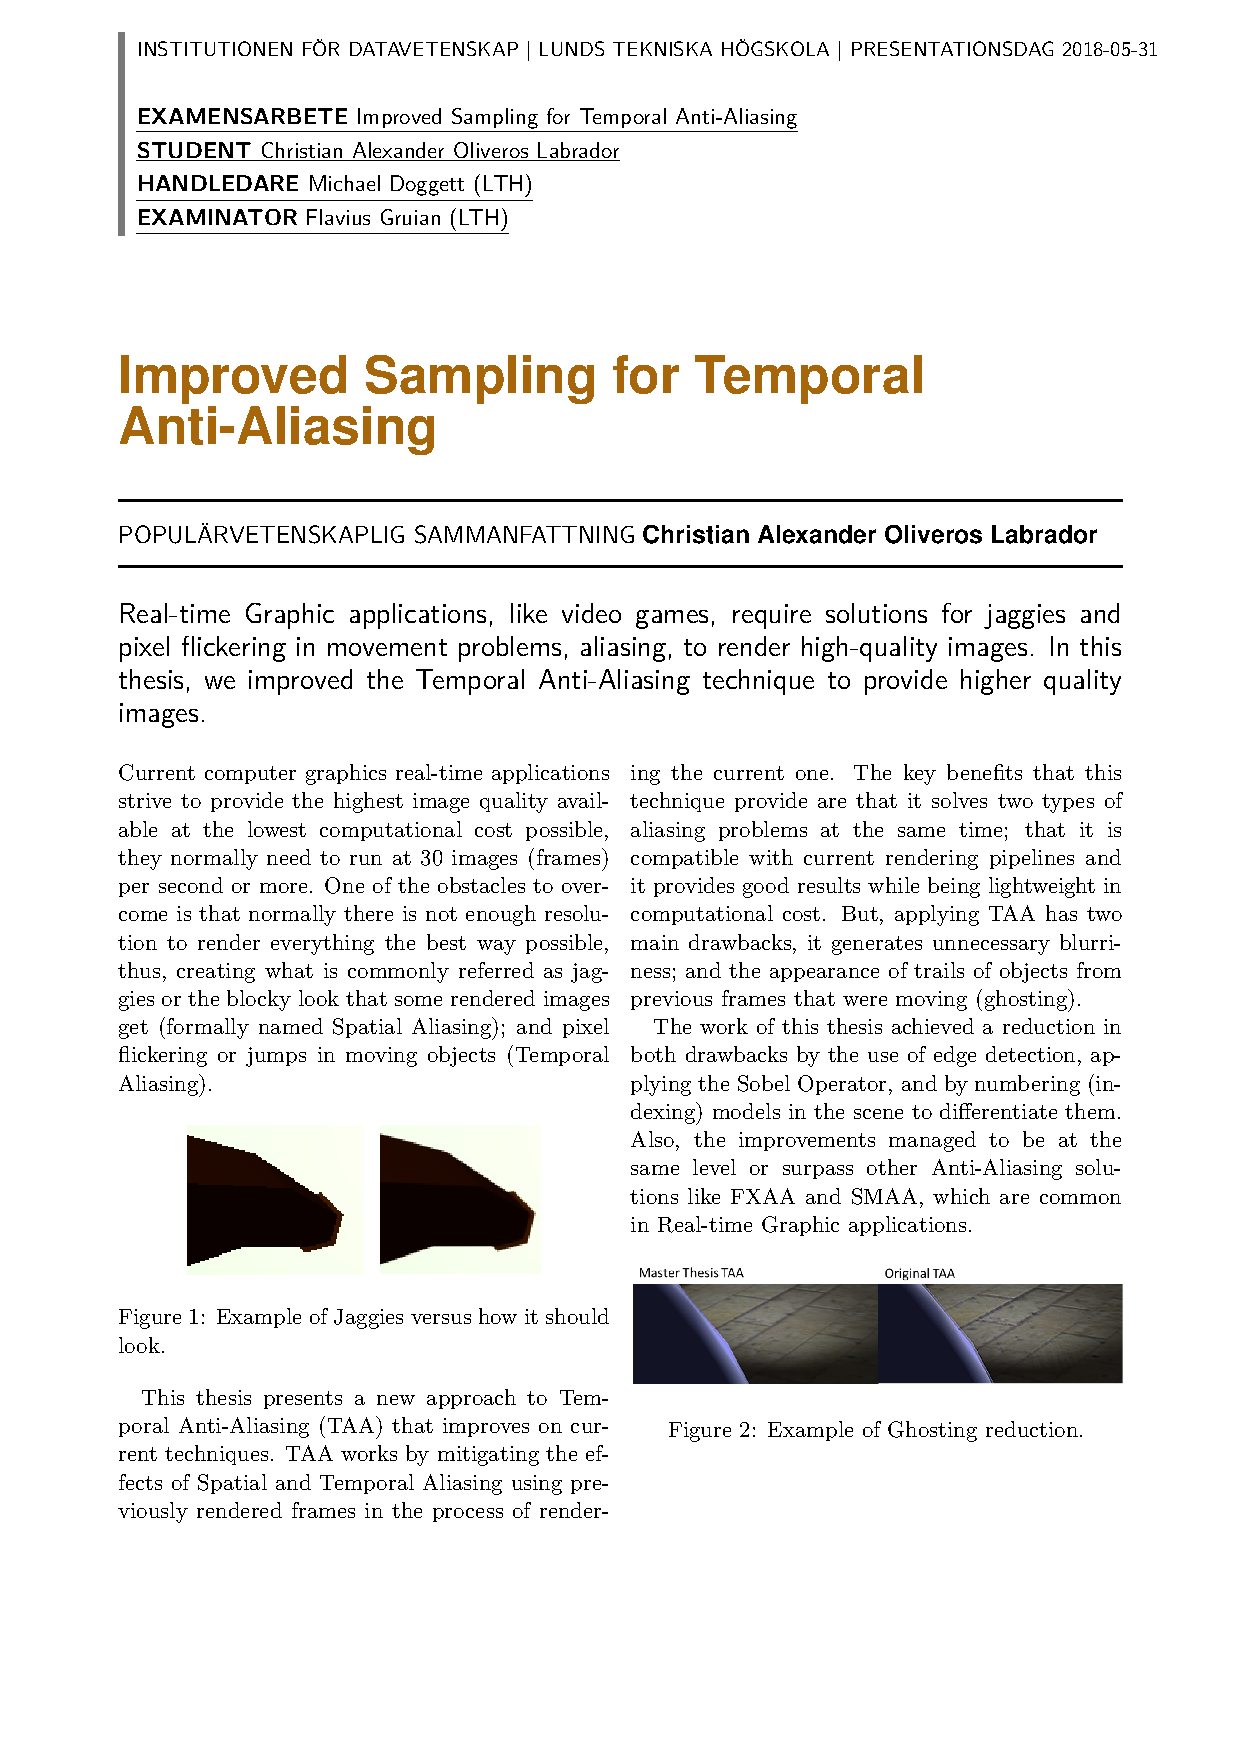
\includepdf[pages={1}]{popsci/popsci.pdf}
\end{appendices}


\end{document}